% !TeX root = ./eLife_supplemental_draft.tex

%%%%%%%%%%%%%%%%%%%%%%%%%%%%%%%%%%%%%%%%%%%%%%%%%%%%%%%%%%%%
%%% ELIFE ARTICLE TEMPLATE
%%%%%%%%%%%%%%%%%%%%%%%%%%%%%%%%%%%%%%%%%%%%%%%%%%%%%%%%%%%%
%%% PREAMBLE
\documentclass[9pt,lineno]{elife}
% Use the onehalfspacing option for 1.5 line spacing
% Use the doublespacing option for 2.0 line spacing
% Please note that these options may affect formatting.
% Additionally, the use of the \newcommand function should be limited.

\usepackage{lipsum} % Required to insert dummy text
\usepackage[version=4]{mhchem}
\usepackage{siunitx}
\DeclareSIUnit\Molar{M}

%%%%%%%%%%%%%%%%%%%%%%%%%%%%%%%%%%%%%%%%%%%%%%%%%%%%%%%%%%%%
%%% ARTICLE SETUP
%%%%%%%%%%%%%%%%%%%%%%%%%%%%%%%%%%%%%%%%%%%%%%%%%%%%%%%%%%%%

\title{Supplemental material for: Fundamental limits on the rate of bacterial cell division}
\author[1, *]{Nathan M. Belliveau}
\author[2, 3, *]{Griffin Chure}
\author[4]{Christina L. Hueschen}
\author[5]{Hernan G. Garcia}
\author[6]{Jane Kondev}
\author[7]{Daniel S. Fisher}
\author[1, 8]{Julie A. Theriot}
\author[1, 9, $\dagger$]{Rob Phillips}
\affil[1]{Department of Biology, University of Washington, Seattle, WA, USA}
\affil[2]{Division of Biology and Biological Engineering, California Institute of Technology, Pasadena, CA, USA}
\affil[3]{Department of Applied Physics, California Institute of Technology, Pasadena, CA, USA}
\affil[4]{Department of Chemical Engineering, Stanford University, Stanford, CA, USA}
\affil[5]{Department of Molecular Cell Biology and Department of Physics, University of California Berkeley, Berkeley, CA, USA}
\affil[6]{Department of Physics, Brandeis University, Waltham, MA, USA}
\affil[7]{Department of Applied Physics, Stanford University, Stanford, CA, USA}
\affil[8]{Allen Institute for Cell Science, Seattle, WA, USA}
\affil[9]{Department of Physics, California Institute of Technology, Pasadena, CA, USA}
\affil[$\dagger$]{Address correspondence to phillips@pboc.caltech.edu}
\affil[*]{Contributed equally}

\contrib[*]{These authors contributed equally to this work}

%%%%%%%%%%%%%%%%%%%%%%%%%%%%%%%%%%%%%%%%%%%%%%%%%%%%%%%%%%%%
%%% Supplemental START
%%%%%%%%%%%%%%%%%%%%%%%%%%%%%%%%%%%%%%%%%%%%%%%%%%%%%%%%%%%%

\begin{document}

\maketitle

\newpage
\tableofcontents

\newpage
% \section{Summary of Proteome Data: Experimental Details}
\label{sec:SI_exp_summary}

Here we provide a brief summary of the experiments behind each proteomic data
set. The purpose of this section is to identify how the authors arrived at
absolute protein abundances. In the following section
(Section~\nameref{sec:SI_data_summary}) we will then provide a summary of the
final protein abundance measurements that were used throughout the main text.
Table \ref{tab:datasets} provides an overview of the publications we considered.
These are predominately mass spectrometry-based, with the exception of the work
from \cite{li2014} which used ribosomal profiling, and the fluorescence-based
counting done in \cite{taniguchi2010}.

\begin{table}[bt]
\caption{\label{tab:datasets}Overview of proteomic data sets.}
\begin{tabular}{l l l }
\toprule
Author & Method & Reported Quantity \\
\midrule
Taniguchi \textit{et al.} (2010)  & YFP-fusion, cell fluorescence    & fg/copies per cell      \\
Valgepea \textit{et al.} (2012)   & mass spectrometry                & fg/copies per cell      \\
Peebo \textit{et al.} (2014)      & mass spectrometry                & fg/copies per fl        \\
Li \textit{et al.} (2014)         & ribosomal profiling              & fg/copies per cell $^a$ \\
Soufi \textit{et al.} (2015)      & mass spectrometry                & fg/copies per cell      \\
Schmidt \textit{et al.} (2016)    & mass spectrometry                & fg/copies per cell $^b$ \\
\bottomrule
\end{tabular}

\medskip
a. The reported values assume that the proteins are long-lived compared to the
generation time but are unable to account for post-translational modifications
that may alter absolute protein abundances.
\\
b. This mass spectrometry approach differs substantially from the others since
in addition to the relative proteome-wide abundance measurements, the authors
performed absolute quantification of 41 proteins across all growth conditions
(see Section~\nameref{sec:SI_schmidt} for more details on this).
\end{table}

\subsection{Fluorescence based measurements}
In the work of \cite{taniguchi2010}, the authors used a chromosomal YFP fusion
library where individual strains have a specific gene tagged with a YFP-coding
sequence. 1018 of their 1400 attempted strains were used in the work. A
fluorescence microscope was used to collect cellular YFP intensities across  all
these strains. Through automated image analysis, the authors normalized
intensity measurements by cell size to account for the change in size and
expression variability across the cell cycle. Following correction of  YFP
intensities for cellular autofluorescence, final absolute protein levels were
determined by a calibration curve with single-molecule fluorescence intensities.
This calibration  experiment was performed separately using a purified YFP
solution.

\subsection{Ribosomal profiling measurements}
The work of \cite{li2014} takes a sequencing based approach to estimate protein
abundance. Ribosomal profiling, which refers to the deep sequencing of
ribosome-protected mRNA fragments, can provide a quantitative measurement of the
protein synthesis rate.  As long as the protein life-time is long relative to
the cell doubling time, it is possible to  estimate absolute protein copy
numbers. The absolute protein synthesis rate has units of  proteins per generation,
and for stable proteins will also correspond to the protein  copy number per
cell.

In the experiments, ribosome-protected mRNA is extracted from cell lysate  and
selected on a denaturing polyacrylamide gel for deep sequencing (15–45 nt long
fragments collected and sequenced  by using an Illumina HiSeq 2000 in
\cite{li2014}). Counts of ribosome footprints from the sequencing data were then
corrected empirically for position-dependent biases in ribosomal density across
each gene, as well as dependencies on specific sequences including the
Shine-Dalgarno sequence. These data-corrected ribosome densities represent
relative protein synthesis rates. Absolute protein synthesis rates are obtained
by multiplying the relative rates by the total cellular protein per cell. The
total protein  per unit volume  was determined with the Lowry method to quantify
total protein, calibrated against bovine serum albumin (BSA). By counting
colony-forming units following serial dilution of their cell cultures, they then
calculated the total protein per cell.

\subsection{Mass spectrometry measurements}

Perhaps not surprisingly, the data is predominantly mass spectrometry based. This is
largely due to tremendous improvements in the sensitivity of mass spectrometers,
as well as improvements in sample preparation and data analysis
pipelines. It is now a relatively routine task to extract protein from a cell
and quantify the majority of proteins present by shotgun proteomics. In general, this
involves lysing cells, enzymatically digesting the proteins into short peptide
fragments, and then introducing them into the mass spectrometer (e.g.
with liquid chromatography and electrospray ionization), which itself can
have multiple rounds of detection and further fragmentation of the peptides.

Most quantitative experiments rely on labeling protein with stable isotopes,
which allow multiple samples to be measured together by the mass
spectrometer. By measuring samples of known total protein abundance simultaneously (i.e. one
sample of interest, and one reference), it is possible to determine relative
protein abundances. Absolute protein
abundances can be estimated following the same approach used above for ribosomal
profiling, which is to multiply each relative abundance measurement by the total
cellular protein per cell. This is the approach taken by \cite{valgepea2013} and
\cite{peebo2015}, with relative protein abundances determined based on the
relative peptide intensities (label free quantification 'LFQ' intensities). For
the data of \cite{valgepea2013}, total protein per cell was determined by
measuring  total protein by the Lowry method, and counting colony-forming units
following serial dilution. For the data from   \cite{peebo2015}, the authors did
not determine  cell quantities and instead report the cellular protein
abundances in protein per unit  volume by assuming a mass density of 1.1 g/ml,
with a 30\% dry mass fraction.

An alternative way to arrive at absolute protein abundances is to dope in
synthetic peptide  fragments of known abundance. These can serve as a direct way
to calibrate mass spectrometry  signal intensities to absolute mass. This is the
approach taken by \cite{schmidt2016}. In addition  to a set of shotgun proteomic
measurements to determine proteome-wide relative abundances,  the authors also
performed absolute quantification of  41 proteins covering over four orders of
magnitude in cellular abundance. Here,  a synthetic peptide was generated for
each of the proteins, doped into each protein sample, and used these to
determine absolute protein abundances of the 41 proteins. These absolute
measurements, determined for every growth condition,  were then used as a
calibration curve to convert proteomic-wide relative abundances into  absolute
protein abundance per cell. A more extensive discussion of the
\cite{schmidt2016} data set can be found in Section \nameref{sec:SI_schmidt}.

\section{Summary of Proteomic Data}
\label{sec:SI_data_summary}

In the work of the main text we only used the data from \cite{valgepea2013,
li2014, peebo2015, schmidt2016}. As shown in \FIG{total_protein_final}(A), the
reported total protein abundances in the work of \cite{taniguchi2010} and
\cite{soufi2015} differed quite substantially from the other work. For the work
of \cite{taniguchi2010} this is in part due to a lower coverage in total
proteomic mass quantified, though we also noticed that most proteins appear
undercounted when compared to the other data.

\FIG{total_protein_final}(B) summarizes the total protein mass for each data
point in our final compiled data set. We note that protein abundances were all
scaled so they followed a common growth rate-dependent change in total protein
mass.  While our inclination initally was to leave reported copy numbers
untouched,  a notable descrepency in the scaling total protein per cell between
\cite{schmidt2016} and the other data sets forced us to dig deeper into those
measurements (compare \cite{schmidt2016} and \cite{li2014} data in
\FIG{total_protein_final}(A)). The particular trend in \cite{schmidt2016}
appears to be due to assumptions of cell size and we provide a more extensive
discussion and analysis of that data set in section \nameref{sec:SI_schmidt}. As
a compromise, and in an effort to treat all data equally, we instead scaled all
protein abundance values to a data-driven estimate of total protein per cell.
Here we used cell size measurements from \cite{si2017, si2019}, and an estimate
of total protein content through expected dry mass. Total protein per cell was
estimated using available data on total DNA, RNA, and protein from
\cite{basan2015, dai2016}, which  account for the majority of dry mass in the
cell. We consider these details in sections \nameref{sec:protein_size_SV} and
\nameref{sec:estimate_protein_per_cell} that follows.

\begin{figure*}
    \centering{
        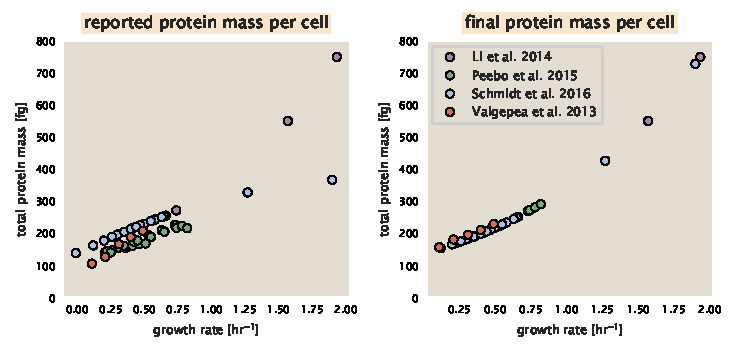
\includegraphics{SI_figs/dataset_corrections.pdf}
        \caption{\textbf{Summary of the growth-rate dependent total protein
        abundance for each data set.} (A) Total protein abundance per cell as
        original reported in the data sets of \cite{taniguchi2010, valgepea2013, li2014,
        soufi2015, peebo2015, schmidt2016}. Note that the data from \cite{peebo2015} only
        reported protein abundances per unit volume and total protein per cell
        was found by multiplying these by the growth-rate dependent cell size as
        determined by \cite{si2017}. (B) Adjusted total protein abundances
        across the proteomic data sets are summarized. Protein abundances were
        adjusted so that all data shared a common set of growth-rate dependent
        total protein per cell and cellular protein concentration following the
        cell size expectations of \cite{si2017} (see section on
        \nameref{sec:protein_size_SV} for further details). }
        \label{fig:total_protein_final}
    }
\end{figure*}

Lastly, in \FIG{upset} we show the total proteomic coverage and overlap of
proteins quantified across each data set. Here we have used  an UpSet diagram
\citep{Lex2014} to compare the data. Overall, the overlap in quantified proteins
is quite high, with 1157 proteins quantified across all data sets. The
sequencing based approach of \cite{li2014} has substantially higher coverage
compared to the mass spectrometry data sets (3394 genes versus the 2041 genes
quantified in the work of \cite{schmidt2016}). However, in terms of total
protein mass, the data from \cite{li2014, schmidt2016, peebo2015} each quantify
roughly equivalent total protein mass.  An exception to this is in the data from
\cite{valgepea2013}, where we find that  the total protein quantified in
\cite{valgepea2013} is 90-95 \% of the total protein mass (when using the data
from \cite{schmidt2016} as a reference).


\begin{figure*}
    \centering{
        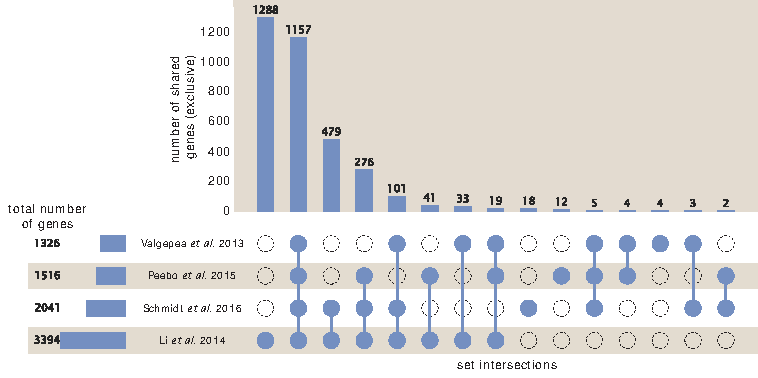
\includegraphics{SI_figs/dataset_upset_diagram.pdf}
        \caption{\textbf{Comparison of proteomic coverage across different data sets.}
        An UpSet diagram \citep{Lex2014} summarizes the total number of protein
        coding genes whose protein abundance was reported in the data sets of
        \cite{valgepea2013, li2014, schmidt2016, peebo2015}. The total number
        of genes reported in each individual data set are noted on the bottom
        left, while their overlap  is summarized in the bar chart. Each column
        here refers to the intersection of a set of data sets  identified by
        blue circles.
        } \label{fig:upset}
    }
\end{figure*}

% \section{Summary of final compiled data set.}

[NB: in progress]

% NB: need to make summary figure with 2x2 panels; top row A) reported total protein per cells
% B) protein concentration. bottom row, C) new total protein mass per cell,
% C) new protein concentration.

% NB: It may be helpful to appeal to the 'classic growth laws' early on in this text
% as a rational to guide thinking with expectations about total cell mass, cell volume w.r.t.
% growth rate.
%
% The data sets encompass a wide range of bacterial growth conditions and
% different \textit{e. coli} strains. In order to determine protein abundance on a
% cell basis,  different strategies  were taken to determine cell counts and cell
% volume. It was therefore important to consider if any obvious discrepancies
% exist across the data and whether these might be reasonably dealt with to make
% the compiled data set internally consistent. \textit{a priori}, there are
% well-documented observations about how characteristics such as total protein
% mass per cell and cell volume  should scale with growth rate. We were therefore
% inclined to only renormalize data in a  way  that was consistent with
% expectations.
% In this section we describe the data manipulations that were applied to those originally reported.
%

%
% Figure [](A) compares the total protein mass reported as a function of
% growth rate for each of the original data sets, while in Figure \ref[](B)  we
% plot the final values that were used in this work. A .csv file containing
% protein copy numbers per cell and mass per cell across all data sets is available for download on our
% GitHub repository.

% \section{Adjustments to Schmidt \textit{et al.} dataset}
\label{sec:SI_schmidt}

% NB: It may be useful to note that none of this should have any effect on the relative
% abundances found in each dataset.

While the dataset from Schmidt \textit{et al.} remains a heroic effort that our lab
continues to return to as a resource,
there were steps taken in their calculation of protein copy number
that we felt needed some further consideration. In particular, the authors made an assumption of
constant cellular protein concentration across all growth conditions and
used measurements of cell volume that appear inconsistent with an expected
exponential scaling of cell size with growth rate that is well-documented in
\textit{E. coli} (\cite{schaechter1958, taheriaraghi2015, si2017}).

We begin by looking at their cell volume measurements, which are shown in blue in Figure \ref{fig:cell_size_literature}.
As a compairon, we also plot cell sizes reported in three other recent papers:
measurements from Taheri-Araghi \textit{et al.} and Si \textit{et al.} come from
the lab of Suckjoon Jun, while those from Basan \textit{et al.} come  from the lab
of Terence Hwa.  Each set of measurements used microscopy and cell segmentation to determine the
length and width, and then calculated cell size by treating the cell is a
cylinder with two hemispherical ends. While there is a large discrepancy in cell
size between the two research groups, Basan \textit{et al.} found that this came
specifically from uncertainty in determining the cell width, which is prone to
inaccuracy given the small cell size and optical resolution limits (further described in their supplemental text). Perhaps the
more concerning point is that while each of these alternative measurements show
an exponential increase in  cell size at faster growth rates, the
measurements used by Schmidt \textit{et al.} appear to plateau. This resulted in an analogous trend in their final reported total
cellular protein per cell as shown in Figure \ref{fig:schmidt_adjustment_summary} (purple data points),
 and is in disagreement with other measurements of total protein at these
 growth rates (\cite{basan2015}).

\begin{figure}
		\centering{
    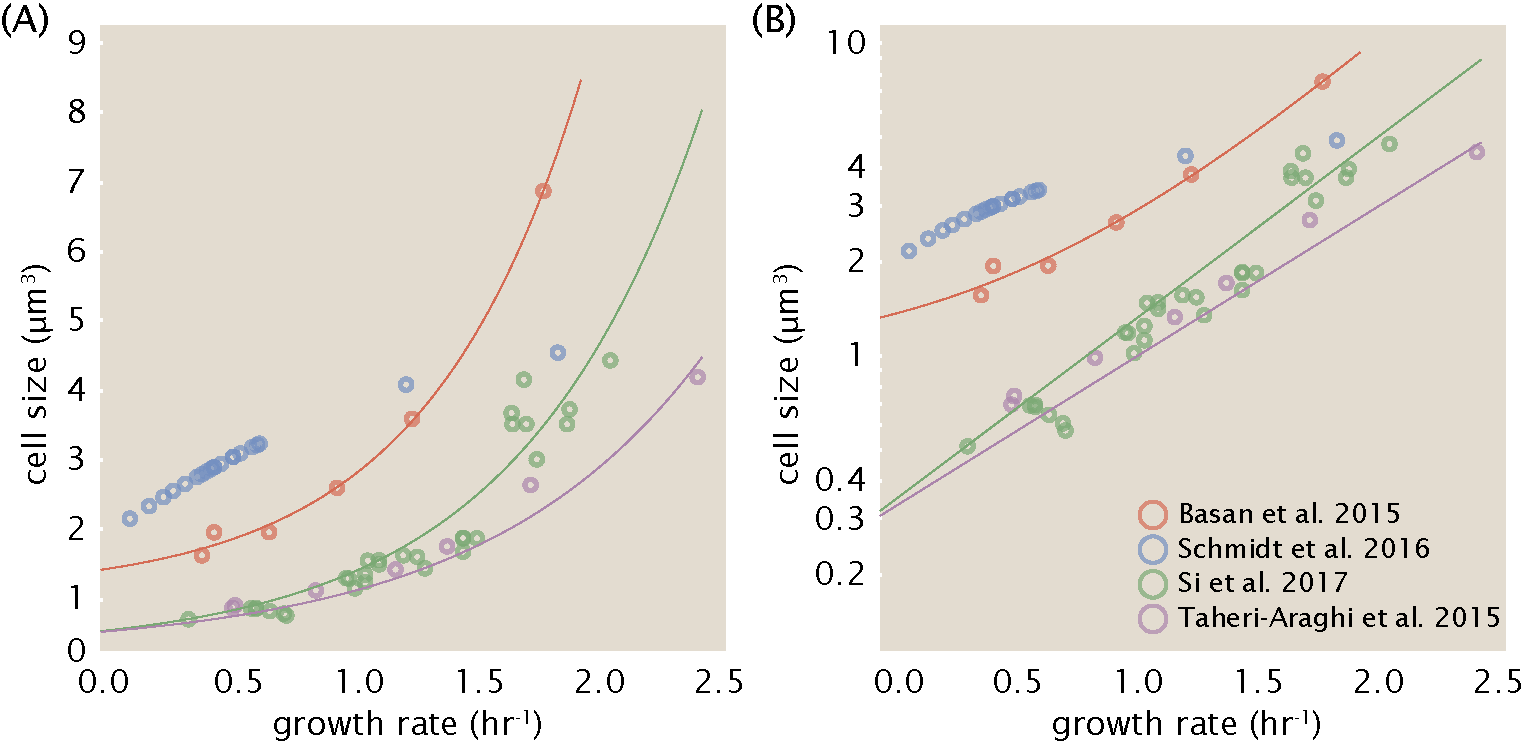
\includegraphics[width=1\textwidth]{SI_figs/supplemental_cell_volumes.pdf}
  \caption{\textbf{Measurements of cell size as a function of growth rate.}
	 	(A) Plot of the reported cell sizes from several recent papers.  The data
	 	in blue come from Volkmer and Heinemann, 2011 (\cite{Volkmer2011}) and were
	 	used in the work of Schmidt \textit{et al.}. Data from the lab of Terence Hwa
	 	are shown in red (\cite{basan2015}), while the two data sets shown in green
	 	and purple come from the lab of Suckjoon Jun (\cite{taheriaraghi2015,
	 	si2017}). (B) Same as in (A) but with the data plotted on a logarithmic
	 	y-axis to highlight the exponential scaling that is expected for \textit{E.
	 	coli}.}
  \label{fig:cell_size_literature}
  }
\end{figure}

Since it is not obvious how measurements of cell size might have influenced
their reported protein abundances, we will go through this calculation in the
next section. We will also show how these can adjusted to better reflect the
alternative measurements of cell size shown in Figure
\ref{fig:cell_size_literature}. Finally, we consider several strategies to
adjust the reported copy numbers, with the result summarized in Figure
\ref{fig:schmidt_adjustment_summary}. For most growth conditions, we find that
total protein expectations are not expected to change dramatically. However, for
the fastest growth conditions, with glycerol + supplemented amino acids, and LB
media, there is quite a bit of variability among are different estimates.



%
% The need for an
% In the next three subsections we consider three different approaches to rescale
% the reported protein abundances from Schmidt \textit{et al.} to make them
% consistent with our expectation that cell size and total protein should increase
% exponentially with growth rate.  Figure [] summarizes Ultimately, we find that
% each approach leads to a similar result, with absolute abundances only changing
% substantially in the fastest growth conditions, in LB media and M9 minimal media
% + glycerol and amino acid supplement.

\begin{figure}
		\centering
    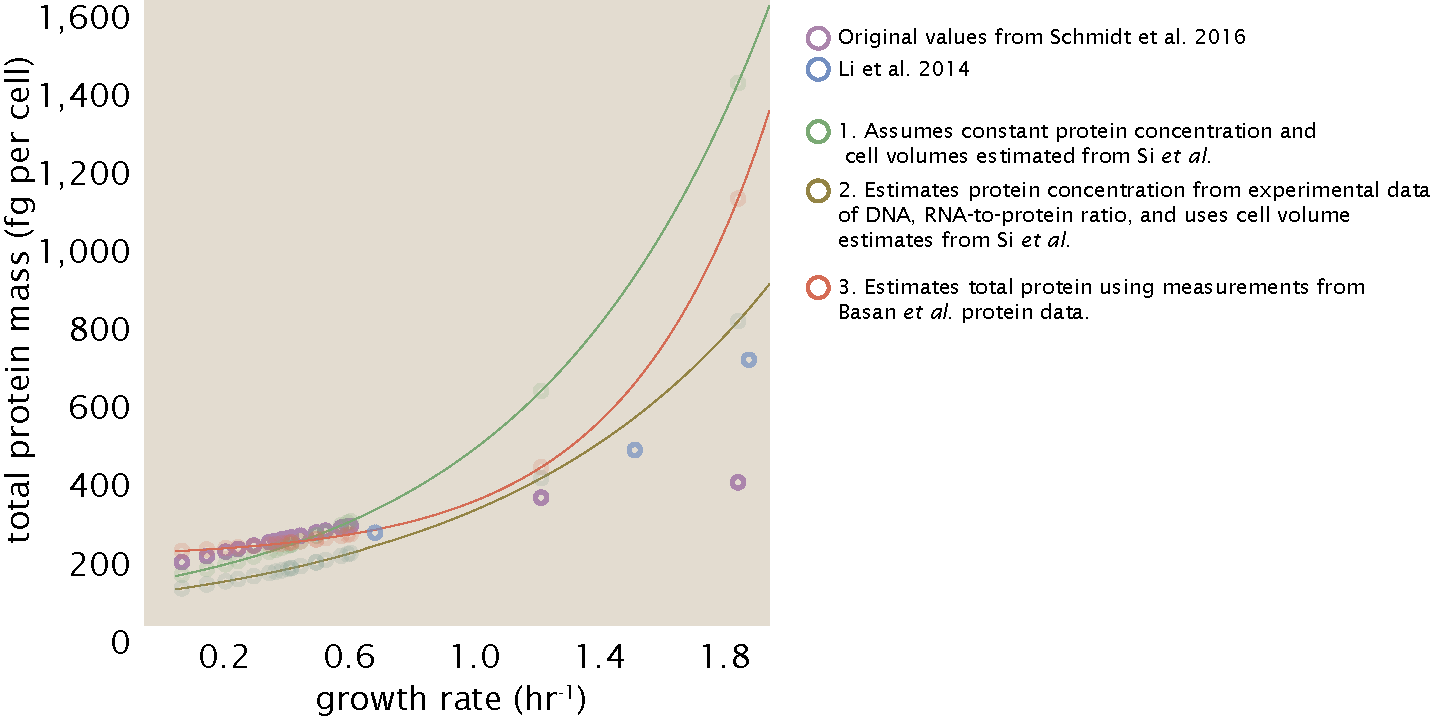
\includegraphics[width=1\textwidth]{SI_figs/schmidt_protein_corrections.pdf}
  \caption{{\bf Alternative estimates of total cellular protein for the growth conditions considered in Schmidt \textit{et al.}} The original protein mass from Schmidt \textit{et al.} and Li \textit{et al.} are shown in purple and blue, respectively. \textit{Green}: Rescaling of total protein mass assuming a growth rate independent protein concentration and cell volumes estimated from Si \textit{et al.} 2017.
  \textit{Gold}:  Rescaling of total protein mass using estimates of growth rate-dependent protein concentrations and cell volumes estimated from Si \textit{et al.} 2017.
  \textit{Red}: Rescaling of total protein mass using the experimental measurements from Basan \textit{et al.} 2015.
	 	}
  \label{fig:schmidt_adjustment_summary}
\end{figure}

\subsection{Effect of cell volume on reported absolute protein abundances in the work of Schmidt \textit{et al.} .}

The authors calculated proteome-wide  protein abundance by first determining
absolute abundances of 41 pre-selected proteins, which relied on adding
synthetic heavy reference peptides into their protein samples at known abundance
(with proteins selected to cover the range of expected copy numbers).  This
absolute quantitation was performed in replicate for each growth condition.
Separately, the authors also performed a more conventional mass spectrometry
measurement for samples from each growth condition, which attempted to maximize
the number of quantified proteins but only provided relative abundances based on
peptide intensities. Finally, using their 41 proteins with absolute abundances
already determined, they then created calibration curves with which to relate
their relative intensity to absolute protein abundance for each growth
condition.  This allowed them to estimate absolute protein abundance for all
proteins detected in their proteome-wide data set. Combined with their flow
cytometry cell counts, they were then able to determine absolute abundance of
each protein detected on a per cell basis.

While this approach provided absolute abundances, another necessary step needed
to arrive at total cellular protein is to account for any protein loss during
their various protein extraction steps. Here the authors attempted to determine
total protein separately using a BCA protein assay.  In personal communications,
it was noted that determining reasonable total protein abundances by BCA across
their array of growth conditions  was particularly troublesome. Instead, they
noted confidence in their total protein measurements for cells grown in M9
minimal media + glucose and  used this as a reference point with which to
estimate the total protein for all other growth conditions.

For cells grown in M9 minimal media + glucose an average total mass of $M_P$ =
240 fg per cell was measured. Using their reported cell volume, reported as
$V_{orig}$ = 2.84 fl, a cellular protein concentration of $[M_P]_{orig}$ =
$M_P/V_{orig}$ = 85 fg/fl. Now, taking the assumption that cellular protein
concentration is relatively independent of growth rate, they could then estimate
the total protein mass for all other growth conditions from,

\begin{equation}
	M_{P\_i} = [M_P]_{orig} \cdot V_{i}
\end{equation}
where $M_{P_i}$ represents the total protein mass per cell and $V_{i}$ is the
cell volume for each growth condition $i$ as measured in Volkmer and Heinemann,
2011. Here the thinking is that the values of $M_{P_i}$ reflects the total
cellular protein for growth condition $i$, where any discrepancy from their
absolute protein abundance is assumed to be due to protein loss during sample
preparation. The protein abundances from their absolute abundance measurements
noted above were therefore scaled to their estimates and are  shown in Figure
\ref{fig:schmidt_adjustment_summary} (purple data points).


% Before continuing, it is useful to perform a quick estimate of cellular protein concentration. If we assume a cellular mass
% density of 1.1 g/ml, 30\% dry mass, with 55 \% of the dry mass taken up by
% protein, the expected cellular protein concentration is given by 1.1 g/ml
% x 30 \% x 60 \%, or about 200 fg / fl total protein. The value from of 85 fg/fl used here
% appears quite low.

If we instead consider the cell volumes predicted in the work of Si \textit{et al.},
we again need to take growth in M9 minimal media + glucose as a reference with known total mass,
but we can follow a similar approach to estimate total protein mass for all other growth conditions.
Letting  $V_{Si\_glu}$ = 0.6 fl be the predicted cell volume, the
cellular protein concentration becomes $[M_P]_{Si}$ = $M_P/V_{Si\_glu}$ = 400 fg/fl. The
new total protein mass per cell can then be calculated from,

\begin{equation}
	M_{P\_i}' = [M_P]_{Si} \cdot V_{Si\_i}
\end{equation}
where $M_{P_i}'$ is the new protein mass prediction, and $V_{Si_i}$ refers to the new volume prediction for each condition $i$,
These are shown as [] dots in Figure \ref{fig:schmidt_adjustment_summary}.


\subsection{Reconsidering assumption that protein concentration is constant.}

We next relax the assumption that cellular protein concentration is constant and
instead, attempt to  estimate it using experimental data. Here we first note
that  for across almost the entire range of growth rates considered here,
protein, DNA, and RNA accounted for at least 90 \% of the dry mass in
measurements from the lab of Terence Hwa (\cite{basan2015}). They also found that
the total dry mass concentration was roughly constant across growth conditions.
Under such a scenario, we can calculate the total dry mass concentration for
protein, DNA, and RNA, which is given by 1.1 g/ml x 30 \% x 90 \% or about
$[M_P]$ = 300 fg per fl. Using the cell volume predictions from Si \textit{et
al.}, we can then calculate the associated mass per cell.

However, even if dry mass concentration is relatively constant across growth
conditions, it is not a given that protein concentration should also be
constant. In particular, we know that rRNA increases substantially at faster
growth rates (\cite{dai2016}). This is a well-documented result that arises from
an increase in the fraction of ribosomes at faster growth rates
(\cite{scott2010}). To proceed we will use therefore rely on experimental
measurements of total DNA content per cell that also come from Basan \textit{et al.},
and RNA to protein ratios that were measured in Dai \textit{et al.} (and cover the entire range of growth conditions considered here). These are
reproduced in Figure \ref{fig:schmidt_adjustment_varying_conc}(A) and (B),
respectively.

Assuming that the protein, DNA, and RNA account for 90 \% of the total dry mass,
the protein mass can then determined by first subtracting the experimentally measured DNA mass,  and then using the experimental estimate of the RNA to protein ratio. The total protein per cell is will be related to the summed RNA and protein mass by,

\begin{equation}
	M_{P} = \frac{[M_P + M_{RNA}]}{1 + (RP_{ratio})}.
\end{equation}
$(RP_{ratio}$ refers to the RNA to protein ratio as measured by Dai \textit{et al.}. In Figure \ref{fig:schmidt_adjustment_varying_conc}(C) we plot the estimated cellular concentrations for protein, DNA, and RNA from these calculations, and in Figure \ref{fig:schmidt_adjustment_varying_conc}(D) we plot their total expected mass per cell.

% Here it is worthwhile noting
% that our result again requires us to assume a particular cell volume for each
% growth rate, which we have estimated from the Si \textit{et al.} data.


\begin{figure}
		\centering
    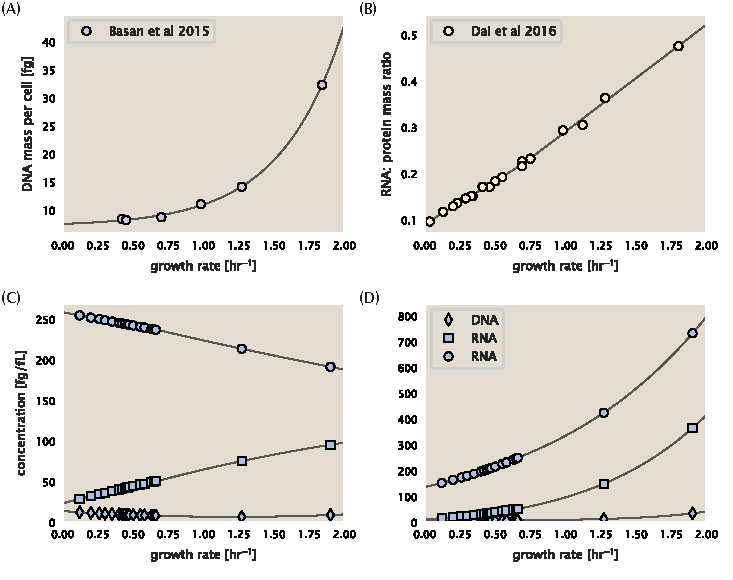
\includegraphics[width=1\textwidth]{SI_figs/schmidt_estimate_protein_RNA_DNA_corrections.pdf}
  \caption{{\bf Empirical estimate of cellular protein, DNA, and RNA as a function of growth rate.} (A) Measured DNA mass per cell as a function of growth rate, reproduced from Basan \textit{et al.} 2015. The data was fit to an exponential curve (DNA mass in fg per cell is given by 0.42 $e^{2.23 \cdot \lambda}$ + 7.2 fg per cell, where $\lambda$ is the growth rate in hr$^{-1}$). (B) RNA to protein measurements as a function fo growth rate. The data was for to two lines: for growth rates below 0.7 hr$^{-1}$, the RNA/protein ratio is 0.18$\cdot \lambda$ + 0.093, while for growth rates faster than 0.7 hr$^{-1}$ the RNA/protein ratio is given by 0.25$\cdot \lambda$ + 0.035. For (A) and (B)
cells are grown under varying levels of nutrient limitation, with cells grown in minimal media with different carbon sources for the slowest growth conditions, and rich-defined media for fast growth rates. (C) Predictions of
cellular protein, DNA, and RNA concentration. (D) Total cellular mass predicted for protein, DNA, and RNA using the cell size predictions from Si \textit{et al.}
	 	}
  \label{fig:schmidt_adjustment_varying_conc}
\end{figure}


\subsection{Estimating cellular protein concentration as a function of growth rate.}

One of the challenges in our estimates in the preceding  sections is the need to estimate protein
concentration and cell volumes. These are inherently difficult to to accurately due to the small size of \textit{E. coli}. Indeed, for
all the additional measurements of cell volume included in Figure \ref{fig:cell_size_literature},
no measurements were performed for cells growing at rates below 0.5 $hr^{-1}$. It therefore remains
to be determined whether our extrapolated cell volume estimates are appropriate, with the
possibility that the logarithmic scaling of cell size might break down for slower growth.

In our last approach we therefore attempt to estimate total protein
using experimental data that required  no estimates of concentration or cell
volume. Specifically, in the work of  Basan \textit{et al}, the authors measured total protein
per cell for a broad range of growth rates (reproduced in Figure \ref{fig:schmidt_adjustment_basan}).
These were determined
by first measuring bulk protein from cell lysate, measured by the colorimetric Biuret method (\cite{You2013}), and then abundance per cell was calculated from cell counts from either plating cells or a Coulter counter. While it is
unclear why Schmidt \textit{et al.} was unable to take a similar approach, the
results from Basan \textit{et al} appear more consistent with our expectation that cell mass will  increase
exponentially with faster growth rates. In addition, although they do not consider growth rates below
about 0.5 $hr^{-1}$, it is interesting to note that the protein mass per cell appears to plateau to a minimum value at slow growth. In contrast, our estimates using cell volume so far have predicted that total protein mass should continue to decrease slightly for slower growing cells.
By fitting this data to an exponential function dependent on growth rate, we could then estimate the
total protein per cell for each growth condition considered by Schmidt \textit{et al.}.
These are plotted in red in Figure \ref{fig:schmidt_adjustment_summary}.


\begin{figure}
		\centering
    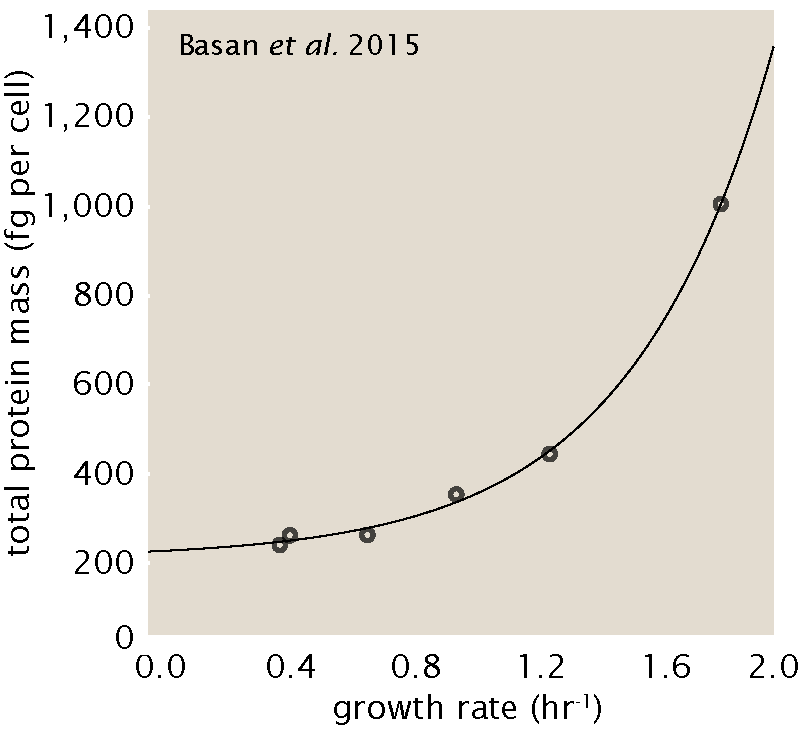
\includegraphics[width=0.5\textwidth]{SI_figs/schmidt_protein_estimate_basan.pdf}
  \caption{{\bf Total cellular protein reported in Basan \textit{et al.} 2015.}
	 	 Measured protein mass as a function of growth rate as reproduced from Basan \textit{et al.} 2015, with cells grown under different levels of nutrient limitation. The data was fit to an exponential curve  where protein mass in fg per cell is given by 14.65 $e^{2,180 \cdot \lambda}$ + 172 fg per cell, where $\lambda$ is the growth rate in hr$^{-1}$).}
  \label{fig:schmidt_adjustment_basan}
\end{figure}

% \section{Peebo {\it et al.}: Conversion from copies/ fL to copies per cell}

In the work of Peebo {\it et al.}, the authors only report protein
concentration. In order to determine protein per cell, we multiple these
concentrations by expected cell volumes  using the predictions from
Taheri-Araghi {\it et al.} This is shown in Figure \ref{}A, where we see that
reported mass is substantially lower than the other work considered here; as
well as work from others [Sinauer, 1990].

Indeed, both Schmidt {\it et al.} and Li {\it et al.} reported a total protein
mass of about 250 fg per cell at a growth rate of about $\lambda \approx 0.5
hr^{-1}$ ( M9 minimal media with glucose and MOPS minimal media, respectively).
Given this discrepancy, in addition to requiring that cellular protein
concentration be internally consistent across the growth conditions they
reported on, we also required that total cellular mass be consistent with the
work Schmidt {\it et al.} and Li {\it et al.} This amounted to performing a
linear regression between total protein mass and growth rate, and using this to
scale the Peebo {\it et al.} dataset according to this trend.

\section{Estimation of cell size and surface area.}

In Figure \ref{fig:cell_size_literature} we looked at a number of recent cell
size measurements and potential issues with the values used by Schmidt
\textit{et al.}. Since most of our data sets lacked any cell size measurements,
we chose instead to use a common set of size measurements for any analysis
that required calculation of cell size or surface area. Here we compile the
cell size measurements from the recent works of Si \textit{et al.} 2017, 2019,
which covers almost the entire range of growth rates considered across the
proteomic data (shown in Figure \ref{fig:final_size_data_Si}). In each dataset,
the authors made measurements on strains MG1655 and NCM3722, which each appear
to show a logarithmic scaling with growth rate.

Since each of our proteomic datasets use either K-12 MG1655 or its derivative
BW25113 (from the lab of Barry L. Wanner; the parent strain of the Keio
collection \citep{datsenko2000, baba2006}), we only considered the MG1655 size
data. The length and width measurements  were well described by 0.5 $e^{1.09
\cdot \lambda}$ + 1.76 $\mu$ m, and 0.64 $e^{0.24 \cdot \lambda}$ $\mu$ m,
respectively. In order to estimate cell size we take the cell as a cylinders
with two hemispherical ends \citep{si2017, basan2015}. Specifically,  cell size
(or volume) is estimated from,

\begin{equation}
V = \pi \cdot r^2 \cdot (l - 2r/3),
\label{eq:cell_size}
\end{equation}
where $r$ is half the cell width. A best fit to the data described by 0.533
$e^{1.037 \cdot \lambda}$ $\mu$ m$^3$. Calculation of the cell surface area is
given by,

\begin{equation}
 S = \eta \cdot \pi (\frac{\eta \cdot \pi}{4} - \frac{\pi}{12})^{-2/3} V^{2/3},
\end{equation}
where $\eta$ is the aspect ratio ($\eta$ = $l/w$) \citep{ojkic2019}.

\begin{figure}
		\centering
    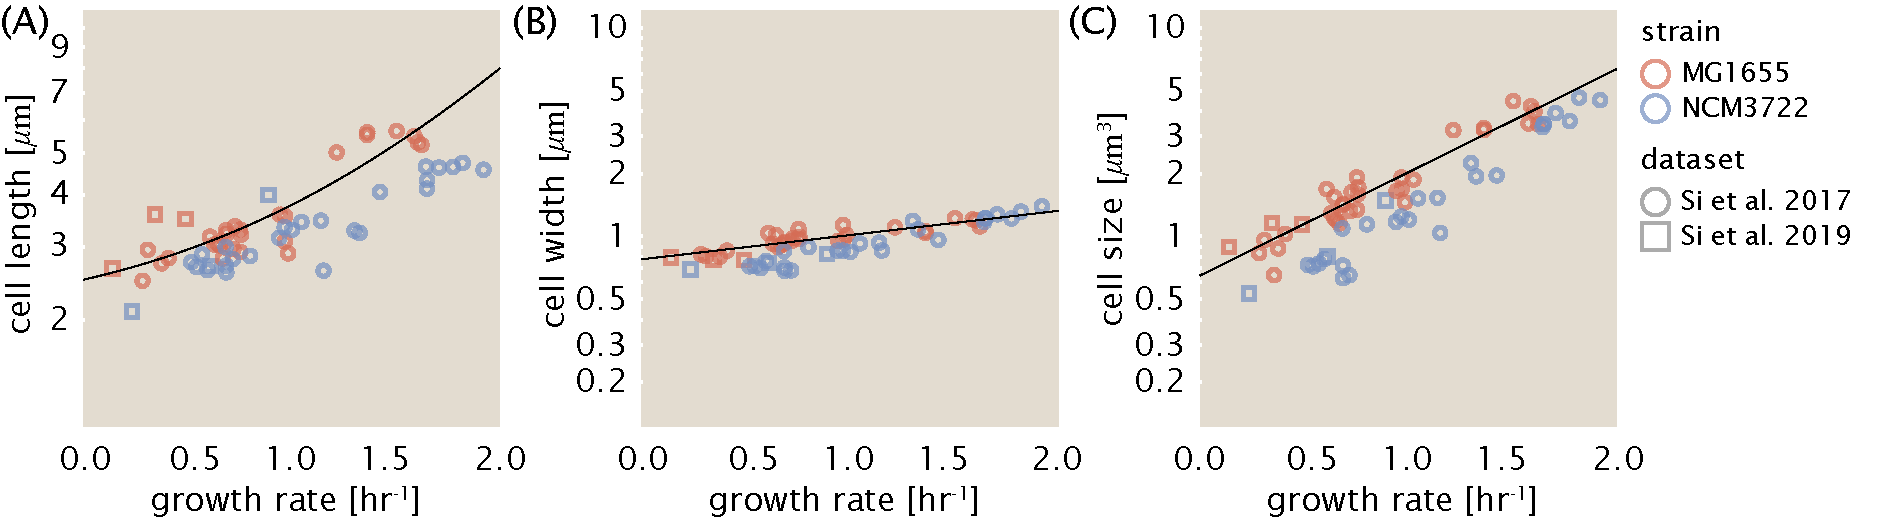
\includegraphics[width=1.0\textwidth]{SI_figs/final_cell_size_Si.pdf}
  \caption{\textbf{Summary of size measurements from Si \textit{et al.} 2017, 2019.}
	 	 Cell lengths and widths were measured from cell contours obtained from
	 	 phase contrast images, and refer to the long and short axis respectively.
	 	 (A) Cell lengths and (B) cell widths show the mean measurements reported
	 	 (they report 140-300 images and 5,000-30,000 for each set of samples;
	 	 which likely means about 1,000-5,000 measurements per mean value reported
	 	 here since they considered about 6 conditions at a time). Fits were made
	 	 to the  MG1655 strain data; length: 0.5 $e^{1.09 \cdot \lambda}$ + 1.76
	 	 $\mu$ m, width:  0.64 $e^{0.24 \cdot \lambda}$ $\mu$ m. (C) Cell size,
	 	 $V$, was calculated as cylinders with two hemispherical ends (Equation \ref{eq:cell_size}). The MG1655 strain data gave a best fit of 0.533 $e^{1.037
	 	 \cdot \lambda}$ $\mu$ m$^3$.}
  \label{fig:final_size_data_Si}
\end{figure}

\section{Extending Estimates to a Continuum of Growth Rates}
In the main text, we considered a standard stopwatch of 5000 s to estimate the
abundance of the various protein complexes considered. In addition to point
estimates, we also showed the estimate as a function of growth rate as
transparent grey curves. In this section, we elaborate on this continuum
estimate and compare and contrast the approach to the point estimate procedure. 

\subsection{Estimation of the total cell mass}
For many of the processes estimated in the main text we relied on a cellular dry
mass of $\approx 300$ fg from which we computed elemental and protein fractions
using knowledge of fractional composition of the dry mass. At modest growth
rates, such as the 5000 s doubling time used in the main text, this is a
reasonable number to use as the typical cell mass is $\approx$ 1 pg and
\textit{E. coli} cells can approximated as 70\% water by volume. However, as we
have shown in this supplemental information, the cell size and therefore cell
volume is highly dependent on the growth rate. This means that a dry mass of 300
fg cannot be used reliably across all growth rates. 


Rather, using 




% \section{Changes to translation under nutrient-limitation.}

In the work of \cite{dai2016}, the authors demonstrated that a number of important
changes take place with respect to translation for cells growing under extents of
nutrient limitation. Specifically, as the growth rate decreases, the translation
elongation rate decreases from a maximum of about 17 aa/s to 8 aa/s in
stationary phase. Addition of sub-lethal doses of chloramphenicol, which bind
to ribosomes and prevent translation, caused an increase in
elongation rate albeit at the consequence of slower growth. Lastly,  for growth
rates below about 0.7 hr$^{-1}$, the measured growth rates were inconsistent
with that required for mass balance of a doubling cell given the independently
measured elongation rates and ribosomal abundance. This suggests that the cell
is also regulating, either actively or passively, the fraction of translating
ribosomes in this nutrient-limited regime.

In that work they propose that there may be a bottleneck in
translation that arises due to lower  availability of ternary complex (TC)
that must bind the ribosome in order for translation to proceed. This complex
consists of aminoacyl-tRNA, elongation factor Tu and guanosine triphosphate.
To account for this bottleneck, they divide the elongation rate into two
coarse-grained timescales: A) binding of the ternary complex to the ribosome,
which will depend inversely on the effective TC concentration $[TC_{eff}]$, and
B) other enzymatic processes that will not depend
on TC concentration. Letting these two timescales be 1/($k_{on} \cdot
[TC_{eff}]$) and 1/$r_t$, the new elongation rate is given by,

\begin{equation}
\frac{1}{r_t} = \frac{1}{k_{on} \cdot [TC_{eff}]} + \frac{1}{r_t^{max}}
\label{eq:rate_dai}
\end{equation}
where $r_t/k_{on}$ is the binding constant of the TC with the ribosome. Further
taking $[TC_{eff}]$ to be proportional to the RNA/protein ratio,

\begin{equation}
[TC_{eff}] = C \cdot (R_m/P_m),
\label{eq:elong_rate}
\end{equation}
they find that  $r_t^{max}$ = 22 aa/s, $k_{on}$ = 6.4 $\mu M^{-1}s^{-1}$, and
$C$ = 31 $\mu M$.

This model does remarkably well in predicting how elongation rate varies  as a
function of ternary complex (assumed proportional to ribosomal content),
irrespective of whether chloramphenicol is present in the media.  In the context
of nutrient limitation however, it provides little intuition into how elongation
rate and growth rate will vary as the media gets poorer. Here, we therefore
consider a scenario where it is the amino acid (and hence aminoacyl-tRNA) that
is limiting in the poorest of growth conditions. Our rationalization for this
choice, instead of example EF-Tu in particular, is that cells are actively
putting away ribosomes at slow growth. If EF-Tu were a limiting component,
wouldn't it be more reasonable for the cell to make fewer ribosomes and
additional EF-Tu to maximize protein synthesis and growth rate? While this
remains speculation, and difficult to determine the validity, we are encouraged
by the mass spectrometry results from \citep{bennett2009}. Cells grown with
acetate had a reduced total amino acid concentration than faster growing cells
with either glucose or glycerol.  This approach nevertheless allows us to gain
some intuition into the consequences of a limiting amino acid pool.

Here we follow a similar approach to that employed by Dai \textit{et al.}, which
is to divide the elongation rate into two coarse-grained timescales. Here we
assume that the elongation rate depends on A) binding of a ternary complex,
which we instead propose depends on a rate-limiting concentration of $[AA]_{eff}$ and,
2) other enzymatic processes that will not depend on $[AA]_{eff}$. The effective
elongation rate is given by the inverse timescales associated with each step,

\begin{equation}
\frac{1}{r_t} = \frac{1}{k_{on} \cdot [AA]_{eff}} + \frac{1}{r_t^{max}}.
\label{eq:rate_dai_2}
\end{equation}
where $r_t$ is the measured elongation rate, $r_t^{max}$ is the maximum
elongation rate, and $r_t^{max}/k_{on}$ is the binding constant $K_d$ of the
ternary complex with the ribosome. Alternatively, we can re-write this in terms
of the binding constant,

\begin{equation}
r_t = \frac{r_t^{max}}{1 + K_d / [AA]_{eff}}.
\label{eq:rate_Kd}
\end{equation}
If we consider only consumption of amino acids by ribosomes, at the steady state
growth ($\frac{d[AA]_{eff}}{dt} = 0$), $[AA]_{eff}$ will be depend on the difference between
the amino acids synthesized $r_{aa} \ \tau$, and those consumed by ribosomes, $R \cdot r_t \ f_a \ \tau$,

\begin{equation}
[AA]_{eff} =  \frac{\tau (r_{aa} - r_t \cdot R \cdot f_a }{V \ N_A}.
\label{eq:aa_}
\end{equation}
The cell volume $V$ and Avogadro's number $N_A$ are needed to get to units of
concentration (i.e. mM). The factor $R \cdot f_a$ reflects the number of
ribosome equivalents that are actively translating and accounts for the
possibility that not all ribosomes are engaged in translation. As the work of
\citep{dai2016} points out, this may be either due to active regulation by the
cell, the result of improperly assembled ribosomes, or abortive ribosomal
products.

As discussed in the main text, the doubling time $\tau$ will depend on how much proteins
must actually be synthesized in order to double the cell. Specifically, $\tau = ln(2)/\lambda =
ln(2) \ N_{aa} / (r_t \ R \ f_a)$. Plugging this, along with Equation \ref{eq:aa_}, into Equation \ref{eq:rate_Kd} we have,

\begin{equation}
[AA]_{eff} =  \frac{\tau (r_{aa} - r_t \cdot R \cdot f_a)}{V \ N_A}.
\label{eq:aa_}
\end{equation}

\begin{equation}
r_t = \frac{r_t^{max}}{1 + \frac{K_d V N_A r_t R f_a}{N_{aa} (r_{aa} - r_t \cdot R \cdot f_a)}}.
\label{eq:rate_Kd_full}
\end{equation}

% We also note another important point given the experimental observation that the
% elongation rate does not drop to zero aa/s at very slow growth. At some point,
% when nutrient conditions are sufficiently poor, ribosomes will be in excess of
% the rate with which the cell can synthesize them. In this regime ribosomes would
% deplete their amino acid supply and be unable to maintain steady-state growth.
% Rather, a bacterium will need to decrease its pool of actively translating
% ribosomes in order to maintain a constant growth rate. This at least provides us
% with some rationalization for why a cell would apparently regulate its fraction
% of ribosomes actively engaged in translation in poor nutrient conditions.

With some algerbraic manipulation we can rewrite this as,

\begin{equation}
r_t =  \frac{r_t^{max}}{1 + \frac{K_d V N_A }{N_{aa} (\frac{r_{aa}}{r_t \cdot R \cdot f_a} - 1)}}.
\label{eq:rate_Kd_full2}
\end{equation}

We see that the elongation rate should indeed depend on the ribosomal abundance,
at least in how it is related to number of ribosomes $R$ ($R \approx \Phi_R
\cdot N_{aa}/ L_R \propto (R_m/P_m) \cdot N_{aa}/ L_R$). However, in contrast to
the model presented by Dai \textit{et al.}, an increase in $R$ (or $R_m/P_m$)
predicts a decrease in $r_t$ since this will lead to a lower $[AA]_{eff}$ (see
Equation \ref{eq:rate_Kd}). This formulation also jibes with an expectation that
the elongation rate would only increase if the synthesis or import of amino
acids keeps pace and surpases the ribosomal demand during protein synthesis.

In Equation \ref{eq:rate_Kd_full2} we see that the elongation rate $r_t$ will
itself depend on $r_t$. In order to solve for $r_t$ explicitly we note that this
is a quadratic equation of $r_t$ and we can solved by finding its roots. These
are given by,

\begin{equation}
r_t = \frac{+/- \sqrt{c^2 + 4 c k r - r cr - r^2} - c - r}{2 (k - 1)},
\label{eq:rt_roots}
\end{equation}
where $c$ = $r_{aa}/ (R*fa)$, $k$ = $N_A V K_d/N_{aa}$, and $r$ = $r_t^{max}$.

For slow growth conditions, the ratio
$N_{aa}/V$ is relatively constant, and


where we can ignore the root containing a negative square root term since this
results in a negative elongation rate.

In the main text we suggest that the increase in $R$ observed at faster growth
rates is in part a consequence of how the cell biases ribosomal gene dosage, and
increases it's overall biomass. Here we also expect $r_{aa}$ to increase in more
nutrient rich media, since it reflects the synthesis rate of amino acids (or
supply rate, when their imported from the media). Conversely, for a specific
growth condition we expect $r_{aa}$ will remain relatively constant if the
number of ribosomes were perturbed. As a test of this hypothesis, we consider
additional data from Dai \textit{et al.} where sub-lethal doses of
chloramphenicol were added to the media. In these experiments,  they measured
the RNA-to-protein ratio $R_m/P_m$, elongation rate $r_t$, and from their
measurements of growth rate inferred $f_a$ from the requirement of mass balance
(i.e. how  much time would have been needed to double to cell contents given
their measured elongation rate). In order to estimate the number of active
ribosomes here, and in Figure 7 of the main text, we have calculated the
ribosomal mass fraction using their reported RNA-to-protein ratios ($\Phi_R
\approx 2.1 \cdot R_m/P_m$ \cite{dai2016}) and then estimated the number of
active ribosomes from $R \cdot f_a \approx (\Phi_R \cdot N_{aa}/ L_R) \cdot
f_a$.



Figure \ref{fig:Dai_data_Cm} shows this data, along with dashed lines of
constant $r_aa$ based on Equation \ref{eq:rt_roots}. Consistent with our
hypothesis, we find that the fraction of active ribosomes and elongation rate
vary along line of roughly constant $r_aa$ for each growth condition. This is
even though cells were found to increase their RNA-to-protein ratio with
increasing concentrations of chloramphenicol. One point of caution here is that
since the ribosomal fraction ($\propto$ R_m/P_m ratio) was found to vary with
chloramphenicol concentration, other changes in the proteomic composition are
expected and it is unclear whether this might lead to a different value of
$r_aa$. Further experimental work would be needed to more carefully test our
predictions under perturbations like that performed with chloramphenicol.

As a final point, it is now possible to consider how the translation-limited
growth rate  might vary as the parameters $R, f_a$, and $r_t$ by using Equation
1 from the main text. This is re-written here for convienence,

\begin{equation}
\lambda_{\textrm{translation-limited}} \approx \frac{ln(2) \cdot r_t}{L_R}  \Phi_R.
\end{equation}
In the slow growth regime ($\appox$ 0.5 $hr^{-1}$ or slower), $\Phi_R$ does not
vary as dramatically as at fast growth and  in Figure 7(E) of the main text we
created a heatmap of growth rate across this parameter space by assuming a
constant value $\Phi_R$=0.13.

% \section{Average protein expression across the chromosome.}

In Figure 7(B) of the main text we plotted the average protein copy number along
\textit{E. coli}'s chromosome using a boxcar averaging (i.e. running average)
window of 0.5 Mb. This means that at each position on the chromosome, proteins
with a transcription start site that were +/- 0.25 Mb from that position
were  included in the calculated average. For \textit{E. coli},
position 0 bp does not correspond the location of the origin and we  keep to
this convention, using the reported positional information from EcoCyc. Since
the chromosome is circular, when calculating the  average at positions  near the
end positions (i.e. near either 0 bp or 4.6 Mb) we include the copy numbers
on opposing ends.  For example, calculating the average for position 0 bp would
include the range from 4.1 Mb to 0.25 Mb).  Here we provide some additional
analysis to show how the absolute copy numbers compare across growth conditions,
as well as the effect of the specific averaging window size.

In the main text we centered each data set according to the mean average in order
to  compare the relative changes in copy number along the length of the
chromosome in each data set. In reality, there is also a correlation between the
total genomic content and protein copy number, which increases at faster growth.
This is shown in Figure \ref{fig:supplemental_boxcar_1}(A), where we plot the boxcar average from each
growth condition without rescaling each about their mean values.

\begin{figure}
    \begin{fullwidth}
        \centering{
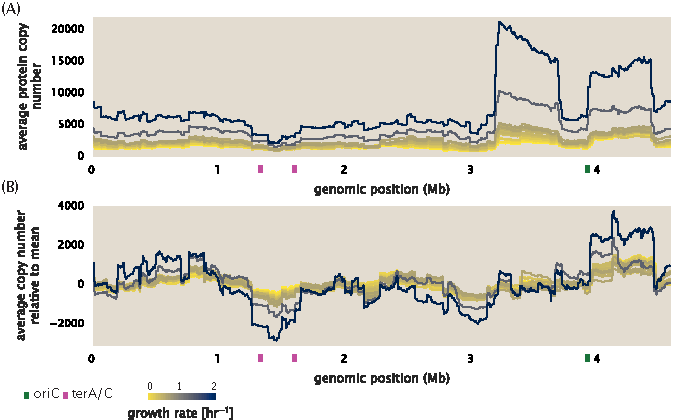
\includegraphics{SI_figs/supplemental_boxcar1.pdf} \caption{\textbf{Position-dependent protein expression at different growth rates.} (A) Protein copy number is reported along the length of the chromosome using a boxcar averaging, with window size of 0.5 Mb.
  (B)The boxcar average protein copy number, shifted relative to the mean value for each
  growth conditions, is show for a window size of 0.5 Mb. In this plot, all ribosomal
  proteins and elongation factor EF-Tu were excluded in the analysis.}
\label{fig:supplemental_boxcar_1} }
\end{fullwidth}
\end{figure}

One of the challenges in interpreting this analysis is that the protein copy
numbers for a small subset of proteins vary dramatically as a function of growth
rate. This is particularly true for ribosomal proteins. In order to check
whether the result is due simply due to the change in ribosomal copy number, we
repeated the analysis with all ribosome proteins, and the translation elongation
factor EF-Tu removed (Figure \ref{fig:supplemental_boxcar_1}(B)). Indeed we still
see a skew in  protein abundance, with higher overall expression at the origin.

The other important parameter in this analysis is the size of the averaging
window, which we took at 0.5 Mb. In Figure \ref{fig:supplemental_boxcar_2} we show
the  results when using averaging window sizes of 0.05 Mb, 0.25 Mb, 0.5 Mb, 1
Mb, and 2 Mb. Aside from the smallest window size of 0.05 Mb, the analysis seems
to show a similar result, with proteins near the origin showing highest
expression. For the window size of  0.05 Mb, the copy numbers become much
noisier due to the large differences in protein copy number  that are observed
irrespective of the specific growth rate.

\begin{figure}
    \begin{fullwidth}
        \centering{
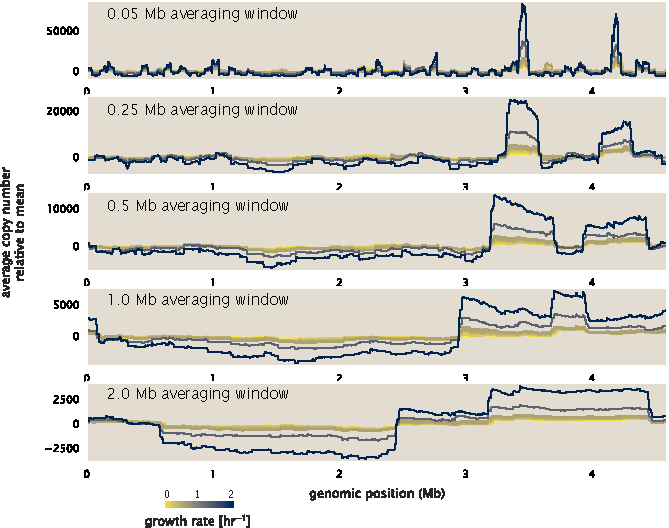
\includegraphics{SI_figs/supplemental_boxcar2.pdf} \caption{\textbf{Position-dependent protein expression at different growth rates.} (A) Protein copy number is reported along the length of the chromosome using a boxcar averaging. Here we consider different averaging window sizes:
0.05 Mb, 0.25 Mb, 0.5 Mb, 1.0 Mb, and 2 Mb. }
\label{fig:supplemental_boxcar_2} }
\end{fullwidth}
\end{figure}

\section{Estimation of $\langle$\#ori$\rangle$ / $\langle$\#ter$\rangle$ and $\langle$\#ori$\rangle$.}

In the main text we consider the possibility that cells are varying their
chromosomal content in order to increase ribosomal content, which will otherwise
become limiting due to the maximal rRNA production per rRNA gene copy. While it is
difficult to show a causal relationship, under such a scenario we nonetheless
expect the ribosomal content to vary with the particular state of DNA
replication. In particular, we can expect that the $\langle$\#ori$\rangle$ /
$\langle$\# ter$\rangle$ ratio will reflect the skew in gene dosage for genes
near the origin and therefore should relate to the relative abundance of
ribosomes that are present closer to the origin.  $\langle$\#ori$\rangle$ is
also useful to consider since it will reflect the total DNA content in the cell
and therefore should relate to the total ribosomal abundance.

In order to estimate the $\langle$\#ori$\rangle$ / $\langle$\# ter$\rangle$
ratio, and $\langle$\#ori$\rangle$, we made use of the measurements  from   Si
\textit{et al.} (2017). We consider their measurements of DNA replication time
($t_{C}$, 'C' period of  cell division), total cell cycle time ($t_{cyc}$, 'C' +
'D' period of cell division), and doubling time $\tau$ from wild-type \textit{E.
coli} growing across a range of growth conditions.

We begin by considering $\langle$\#ori$\rangle$. If the cell cycle time takes
longer  than the time of cell division, the cell will need to initiate DNA
replication  more often than its rate of division, $2^{\lambda t} = 2^{ln(2)
\cdot t/ \tau}$. Cells will need to do in in proportion to the ratio
$\lambda_{cyc} / \lambda =  t_{cyc}/\tau$, and the average number of origins per
cell is then given by $2^{t_{cyc}/ \tau}$.  The average number of termini will
in contrast depend on the lag time between  DNA replication and cell division,
$t_{D}$, with $\langle$\#ori$\rangle$ / $\langle$\# ter$\rangle$ ratio =
$2^{t_{cyc}/ \tau - t_{D}/ \tau} =  2^{t_{C}/ \tau}$.

In Figure \ref{fig:Si_Cm}(A) and (B) we plot the measured $t_{C}$ and $t_{cyc}$ values
versus the doubling time from Si \textit{et al.} data. The authors estimated
$t_{C}$ by marker frequency analysis using qPCR, while  $t_{cyc} = t_{C} +
t_{D}$ were inferred from $t_{C}$ and $\tau$. In the plots we see that both
$t_{C}$ and $t_{cyc}$ reach a minimum  at around 40 and 75 minutes,
respectively. For a C period of 40 minutes, this would correspond to a maximum
rate of elongation of about 1,000 bp/sec. Since we lacked a specific model to
describe how each of these parameters vary with growth condition, we assumed
that they were linearly dependent on the doubling time. For each parameter,
$t_{C}$ and $t_{cyc}$, we split them up into two domains corresponding to poorer
nutrient conditions and rich nutrient conditions ($\tau \approx$ 55 minutes).
The fit lines are shown as solid black lines. In Figure \ref{fig:Si_Cm}(C) and (D) we also
show $t_{C}$ and $t_{cyc}$ as a function of growth rate $\lambda$ along with our
piecewise linear fits, which match the plots in the main text.


\begin{figure}
    \begin{fullwidth}
        \centering{
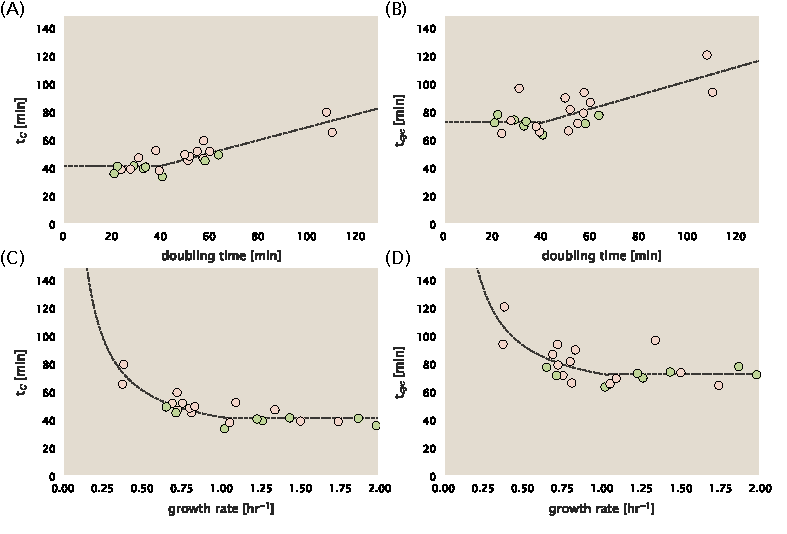
\includegraphics{SI_figs/supplemental_ori_ter.pdf} \caption{\textbf{Estimation of
    $\langle$\#ori$\rangle$ / $\langle$\# ter$\rangle$ and
    $\langle$\#ori$\rangle$ using data from Si \textit{et al.} (2017).} (A) and
    (B) plot the reported $t_{C}$ and $t_{cyc}$ as a function  of cell doubling
    time $\tau$, respectively. The dashed lines show a piecewise fit to  the
    data. For short doubling times (rich media), $t_{C}$ and $t_{cyc}$ are
    assumed  constant. At the transition, taken to occur at 40 minutes, the
    dashed line corresponds  to an assumed proportional increase in each
    parameter as a function of the doubling time. (C) and (D) plot the same data
    as in (A) and (B), but as a function of growth rate, given by $\lambda = ln(2)/\tau$.}
\label{fig:Si_tC_tcyc} }
\end{fullwidth}
\end{figure}



\section{Hypothesis for increase in ribosomal abundance in the presence of chloramphenicol.}

In the main text we note that the observed increase in ribosomal abundance  upon
addition of non-lethal concentrations of chloramphenicol may in part  be a
consequence of limiting rRNA production. Specifically, the proposal assumes that
RNA polymerase are producing rRNA at their maximal rate (i.e. maximal packing of
RNA polymerase on each rRNA operon). By sequestering ribosomes there will be a
decrease in protein synthesis rate (i.e. lower $r_t \cdot R$) and a
corresponding increase in doubling time. Qualitatively then, we may then expect
that that more rRNA (and therefore more ribosomes) may be produced for a
specific growth condition and longer doubling times  Figure
\ref{fig:Si_Cm}(A).

Here we consider data from Si \textit{et al.} (2017) where cells were grown in
the presence of sub-lethal levels of chloramphenicol. In Figure \ref{fig:Si_Cm}(B) we
plot measured RNA-to-protein ratios as a function of $\langle$\#ori$\rangle$ /
$\langle$\# ter$\rangle$ (calculated using their reported values of $\tau_C$ and
$\tau$). While the data is relatively noisy, we do see that
increasing concentrations of chloramphenicol is associated with an increased
RNA-to-protein ratios and this appears roughly independent of the particular
$\langle$\#ori$\rangle$ / $\langle$\# ter$\rangle$ ratio.

One challenge in interpreting the data is that the $\langle$\#ori$\rangle$ /
$\langle$\# ter$\rangle$ ratio for a specific growth condition tends to decrease
with increasing concentrations of chloramphenicol (indicated by marker type).
Since the $\langle$\#ori$\rangle$ / $\langle$\# ter$\rangle$ ratio is defined by
the ratio $\tau_C$/ $\tau$, this is likely a reflection of chloramphenicol
slowing down protein production relative to the rate of DNA replication (though,
both $\tau_C$ and $\tau$ increase with added chloramphenicol).

Lastly, using the reported cell size data that was also available, we also
consider how total ribosome copy number varies with growth condition and
chloramphenicol. Here, as a first approaximation we assume that the total
protein per cell will is proportional to cell size (with total protein $\approx$
cell volume x 1.1 g/ml x 30\% dry mass x 55\% protein). We then estimate the
number of ribosomes by multiplying the protein mass by our estimate of the
ribosomal fraction.  Consistent with the apparent generality in how growth
relates to cell size (size $\propto$ $\langle$\#ori$\rangle$) \citep{si2017},
the number of ribosomes per cell collapse  onto a roughly linear trend with
respect to the  $\langle$\#ori$\rangle$ (Figure \ref{fig:Si_Cm}(C)).

That each of the chloramphenicol curves do not collapse onto a single line when
normalized relative to $\langle$\#ori$\rangle$ (Figure \ref{fig:Si_Cm}(D))
may be a reflection of biosynthetic rates increasing overall in richer media.
For protein translation specifically, the rate of translation increases in both
nutrient-limitation \citep{scott2010}, and with increasing concentrations of
chloramphenicol \citep{dai2016} for poorer media (up to maximum of about 17 aa
per second). It may be that other processes, and production of rRNA in
particular may also slow down in poorer media.

\begin{figure}
    \begin{fullwidth}
        \centering{
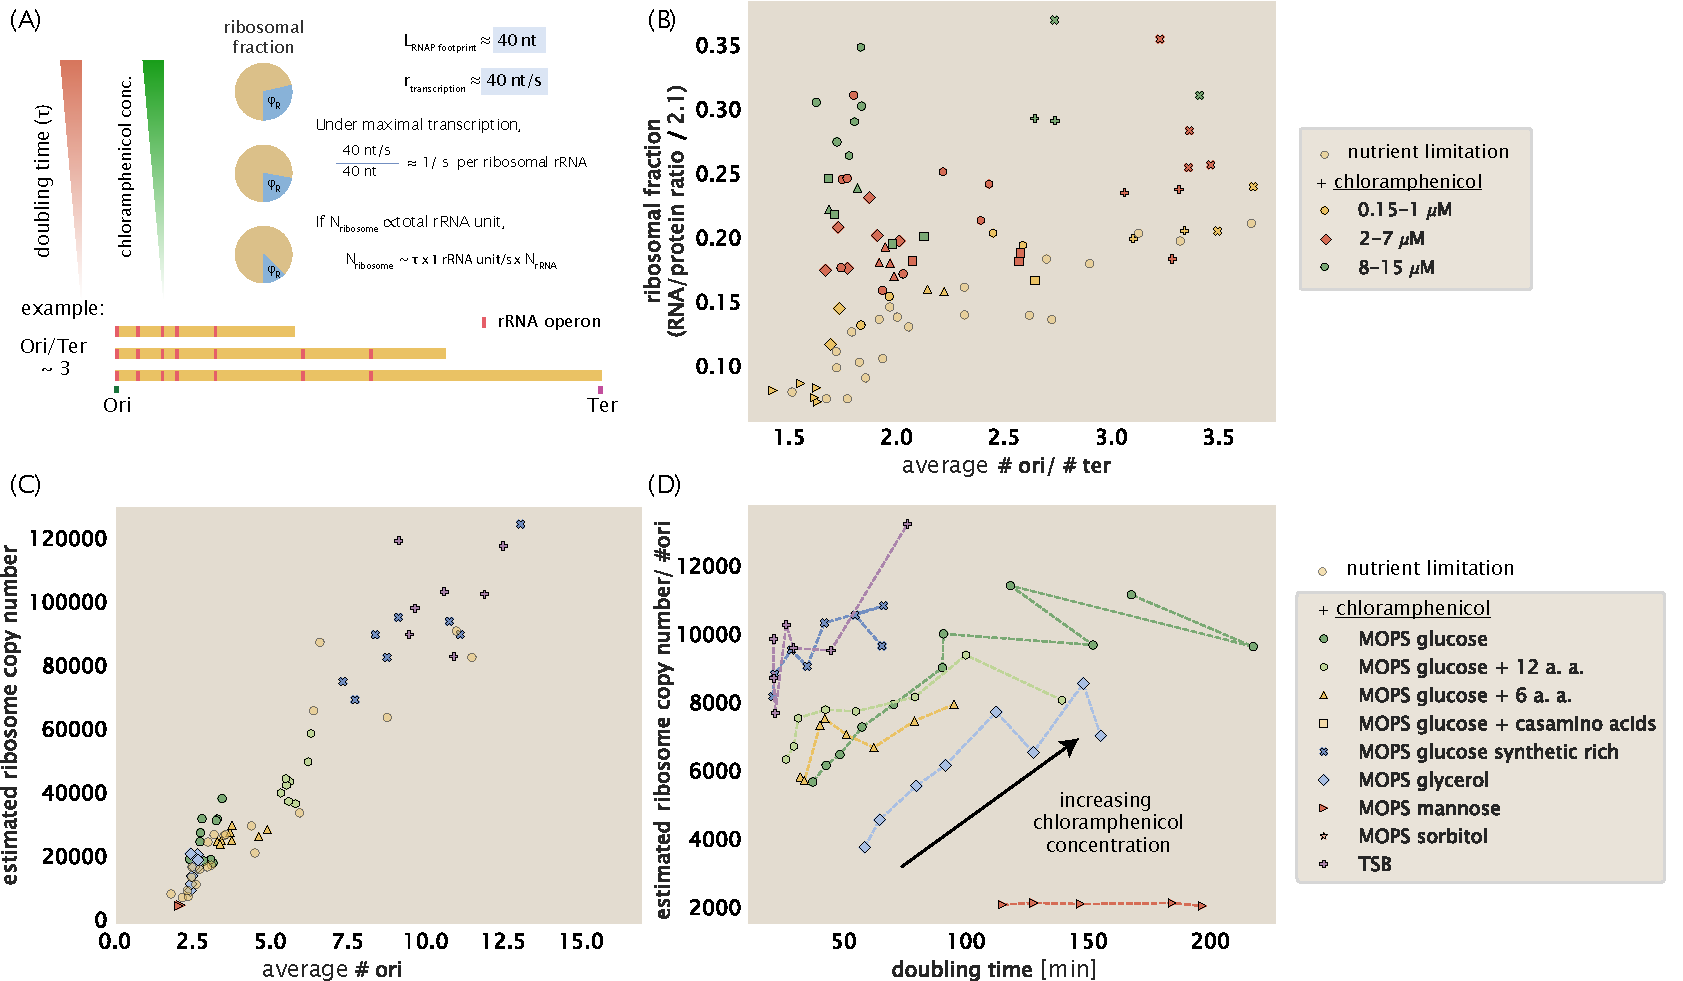
\includegraphics[width=1.2\textwidth]{SI_figs/supplemental_Si_Cm.pdf} \caption{\textbf{Potential effect of
    chloramphenicol on ribosomal abundance of if rRNA production is limiting.}
    (A) Schematic of proposed change in ribosomal abundance upon addition of non-lethal
    does of chloramphenicol. We consider, for example, a $\langle$\#ori$\rangle$ / $\langle$\#ter$\rangle$ ratio of ~ 3, which reflects an effective chromosome whose gene dosage is biased more so to regions near the origin. If ribosome production is limited by
    rRNA production in particular, then sequestering ribosomes will slow down
    cell doubling and provide addition time for more rRNA to be made.
    (B) Estimated ribosomal fraction ($\approx$ RNA/protein ratio x 2.1 \cite{dai2016}) at
    as a function of measured $\langle$\#ori$\rangle$ / $\langle$\# ter$\rangle$ ratio. Data is
    split into 'nutrient-limited' growth (pale yellow), low chloramphenicol concentration (yellow, 0.15 - 1 $\mu$M), medium chloramphenicol concentration (red, 2 - 7 $\mu$M), and
    high chloramphenicol concentration (red, 8 - 15 $\mu$M). Marker type corresponds to
    the growth media as indicated in part (C).
    (C) Scaling of estimated ribosomal copy number with $\langle$\#ori$\rangle$, showing that
    cells still scale their total protein in accord with apparent growth law \citep{si2017}
    irrespective of presence of chloramphenicol.
    (D) Estimated ribosomal copy number normalized by $\langle$\#ori$\rangle$. Data shows
    a media-specific increase in ribosomal abundance per origin with longer doubling times.
    All data is from \citep{si2017}, and show that average values from each growth condition and chloramphenicol concentration (including data from both strains, MG1655 and NCM3722).}
\label{fig:Si_Cm} }
\end{fullwidth}
\end{figure}



\bibliography{library.bib}

%%%%%%%%%%%%%%%%%%%%%%%%%%%%%%%%%%%%%%%%%%%%%%%%%%%%%%%%%%%%
\end{document}
%
